\chapter{Basic concepts}\label{sec:basic_concepts}

UAVCAN is a lightweight protocol designed to provide a highly reliable communication method for
aerospace and robotic applications via the CAN bus.
A UAVCAN network is a decentralized peer network, where each peer (node) has a unique
numeric identifier - \emph{node ID}.
Nodes of a UAVCAN network can communicate using the following communication methods:
\begin{description}
    \item[Message broadcasting] - The primary method of data exchange with publish/subscribe semantics.
    \item[Service invocation] - The communication method for peer-to-peer request/response
    interactions\footnote{Like remote procedure call (RPC).}.
\end{description}

For each type of communication, a predefined set of data structures is used,
where each data structure has a unique identifier - the \emph{data type ID} (DTID).
Some data structures are standard and defined by the protocol specification;
others may be specific to a particular application or vendor.

Since every message or service data type has its own unique data type ID,
and each node in the network has its own unique node ID,
a pair of data type ID and node ID can be used to support redundant nodes with identical
functionality inside the same network.

Message and service data structures are defined using the Data Structure Description Language
(DSDL) (chapter \ref{sec:dsdl}).
A DSDL description can be used to automatically generate the serialization/deserialization code
for every defined data structure in a particular programming language.
DSDL ensures that the worst case memory footprint and computational complexity involved per data type
are constant and easily predictable, which is paramount for hard real-time and safety-critical applications.

On top of the standard data types, UAVCAN defines a set of standard high-level functions including:
node health monitoring, network discovery, time synchronization, firmware update,
plug-and-play node support, and more.
For more information see chapter \ref{sec:application_layer}.

Serialized message and service data structures are exchanged by means of the CAN bus transport
layer (chapter \ref{sec:can_bus_transport_layer}),
which implements automatic decomposition/reassembly of long transfers into/from several CAN frames,
allowing nodes to exchange data structures of arbitrary size.

\begin{figure}[hbt]
    \centering
	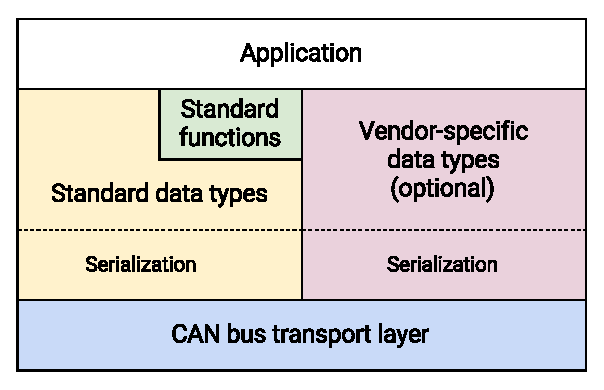
\includegraphics[width=0.5\textwidth]{basic_concepts/Architecture}
	\caption{UAVCAN architectural diagram.\label{fig:architecture}}
\end{figure}

\section{Message broadcasting}

Message broadcasting refers to the transmission of a serialized data structure over the CAN bus to other nodes.
This is the primary data exchange mechanism used in UAVCAN.
Typical use cases may include transfer of the following kinds of data (either cyclically or on an ad-hoc basis):
sensor measurements, actuator commands, equipment status information, and more.

Information contained in a broadcast message is summarized in the table \ref{table:broadcast_message_info}.

\begin{UAVCANSimpleTable}{Broadcast message properties}{|l X|}\label{table:broadcast_message_info}
    Property        & Description \\
    Payload         & The serialized message data structure \\
    Data type ID    & Numerical identifier that indicates how the data structure should be interpreted \\
    Data type major version number & Semantic major version number of the data type description \\
    Source node ID  & The node ID of the transmitting node (excepting anonymous messages) \\
    Transfer ID     & A small overflowing integer that increments with every transfer
                      of this type of message from a given node \\
\end{UAVCANSimpleTable}

\subsection{Anonymous message broadcasting}

Nodes that don't have a unique node ID can publish \emph{anonymous messages}.
An anonymous message is different from a regular message in that it doesn't contain a source node ID.

This kind of data exchange is useful during initial configuration of the node,
particularly during the dynamic node ID allocation procedure\footnote{This is an optional feature.}.

Anonymous messages cannot be decomposed into multiple CAN frames,
meaning that their payload capacity is limited to that of a single CAN frame.
More info is provided in the section \ref{sec:can_bus_transport_layer}.

\section{Service invocation}

Service invocation is a two-step data exchange between exactly two nodes: a client and a server.
The steps are:

\begin{enumerate}
    \item The client sends a service request to the server.
    \item The server takes appropriate actions and sends a response to the client.
\end{enumerate}

Typical use cases for this type of communication include:
node configuration parameter update, firmware update, ad-hoc action request, file transfer,
and similar service tasks.

Information contained in service requests and responses is summarized in the
table \ref{table:service_req_resp_info}.

\begin{UAVCANSimpleTable}{Service request/response properties}{|l X|}\label{table:service_req_resp_info}
    Property        & Description \\
    Payload         & The serialized message data structure \\
    Data type ID    & Numerical identifier that indicates how the data structure should be interpreted \\
    Data type major version number & Semantic major version number of the data type description \\
    Client node ID  & Source node ID during request transfer, destination node ID during response transfer \\
    Server node ID  & Destination node ID during request transfer, source node ID during response transfer \\
    Transfer ID     & A small overflowing integer that increments with every call to this service from a given node \\
\end{UAVCANSimpleTable}

Both request and response contain exactly the same values for all fields except payload,
where the content is application-defined.
Clients match the response with the corresponding request using the following fields:
data type ID, data type major version number, client node ID, server node ID, and transfer ID.
